\subsection{SGX Software Attestation}
\label{sec:sgx_attestation}

The software attestation scheme implemented by SGX follows the principles
outlined in \S~\ref{sec:generic_software_attestation}. An SGX-enabled processor
computes a measurement of the code and data that is loaded in each enclave,
which is similar to the measurement computed by the TPM~(\S~\ref{sec:tpm}). The
software inside an enclave can start a process that results in an SGX
attestation signature, which includes the enclave's measurement and an enclave
message.

However, the software attestation scheme in SGX's design, summarized in
Figure~\ref{fig:sgx_attestation_overview} is unnecessarily complicated by the
decision to deeply couple software attestation with
\textbf{an enclave licensing mechanism that allows Intel to force itself as an
intermediary in the distribution of all enclave software}.

\begin{figure}[hbt]
  \centering
  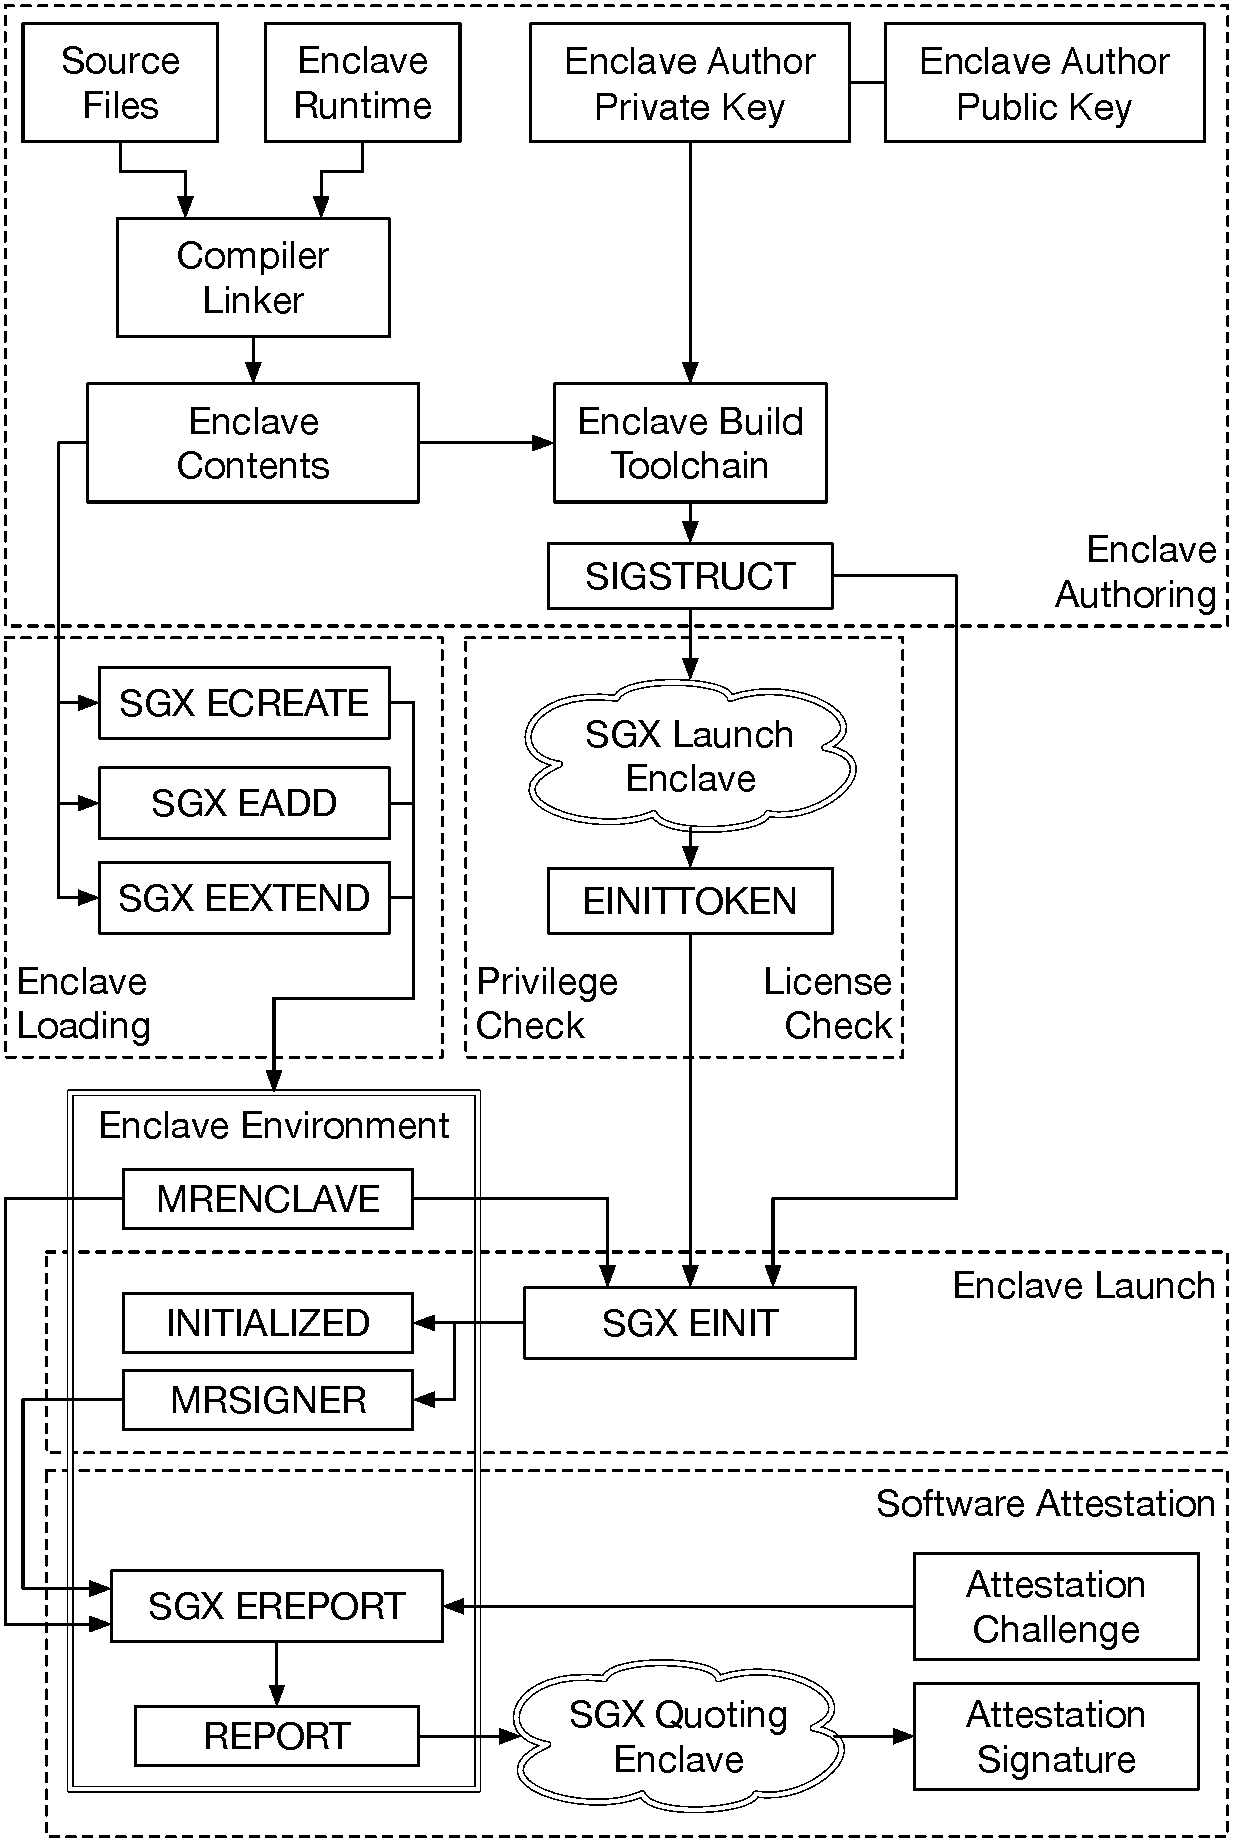
\includegraphics[width=85mm]{figures/sgx_attestation_overview.pdf}
  \caption{
    Setting up an SGX enclave and undergoing the software attestation process
    involves the SGX instructions \texttt{EINIT} and \texttt{EREPORT}, and two
    special enclaves authored by Intel, the SGX Launch Enclave and the SGX
    Quoting Enclave.
  }
  \label{fig:sgx_attestation_overview}
\end{figure}

Under the SGX design, there are two sides to an enclave's identity. The
enclave's measurement, described in \S~\ref{sec:sgx_measurement}, reflects all
the code and data loaded in the enclave when it is initialized. The enclave's
signature, represented as the Signature Structure~(SIGSTRUCT) described in
\S~\ref{sec:sgx_sigstruct}, is an endorsement of the enclave's contents issued
by a software vendor.

Initializing an enclave via \textit{EINIT}~(\S~\ref{sec:sgx_einit_overview})
generally requires an \texttt{EINIT} Token structure~(EINITTOKEN), which can
only be issued by the SGX Launch enclave, as described in
\S~\ref{sec:sgx_launch_enclave}. The SDM does not specify the role of the
Launch Enclave, but one of the SGX patents~\cite{intel2013patent1} discloses in
no uncertain terms that the Launch Enclave is intended to check that the
enclave author has a business relationship with Intel.

After an enclave gets cleared by the SGX Launch Enclave and is initialized via
\texttt{EINIT}, it can authenticate itself to a remote party by participating
in a software attestation process. This is a two-step process. First, the
enclave uses the \texttt{EREPORT} instruction to create a REPORT structure,
described in \S~\ref{sec:sgx_ereport}. This structure only proves the enclave's
identity to the SGX Quoting Enclave, described in
\S~\ref{sec:sgx_quoting_enclave}, which is a special enclave authored by Intel
that can access to the CPU's attestation key. Therefore, the REPORT structure
created by \texttt{EREPORT} is given to the SGX Quoting enclave, which produces
an attestation signature that can be verified by a remote party.

The EINITTOKEN and REPORT structures are passed between enclaves by untrusted
system software, so they require integrity guarantees. The structures'
integrity is assured by a MAC scheme~(\S~\ref{sec:integrity_crypto}) that uses
symmetric keys supplied by the SGX key derivation feature described in
\S~\ref{sec:sgx_egetkey}.


\subsubsection{Enclave Signature}
\label{sec:sgx_sigstruct}
\label{sec:sgx_mrsigner}

% Enclave Signature Structure (SIGSTRUCT): SDM S 38.13

Under the SGX design, an enclave's author must supply a
\textit{Signature Structure}~(SIGSTRUCT), illustrated in
Figure~\ref{sec:sgx_sigstruct}, along with the enclave's contents. The
structure represents a cryptographic endorsement of the enclave's contents, and
associates the enclave with a public key that belongs to its author.

\begin{figure}[hbt]
  \centering
  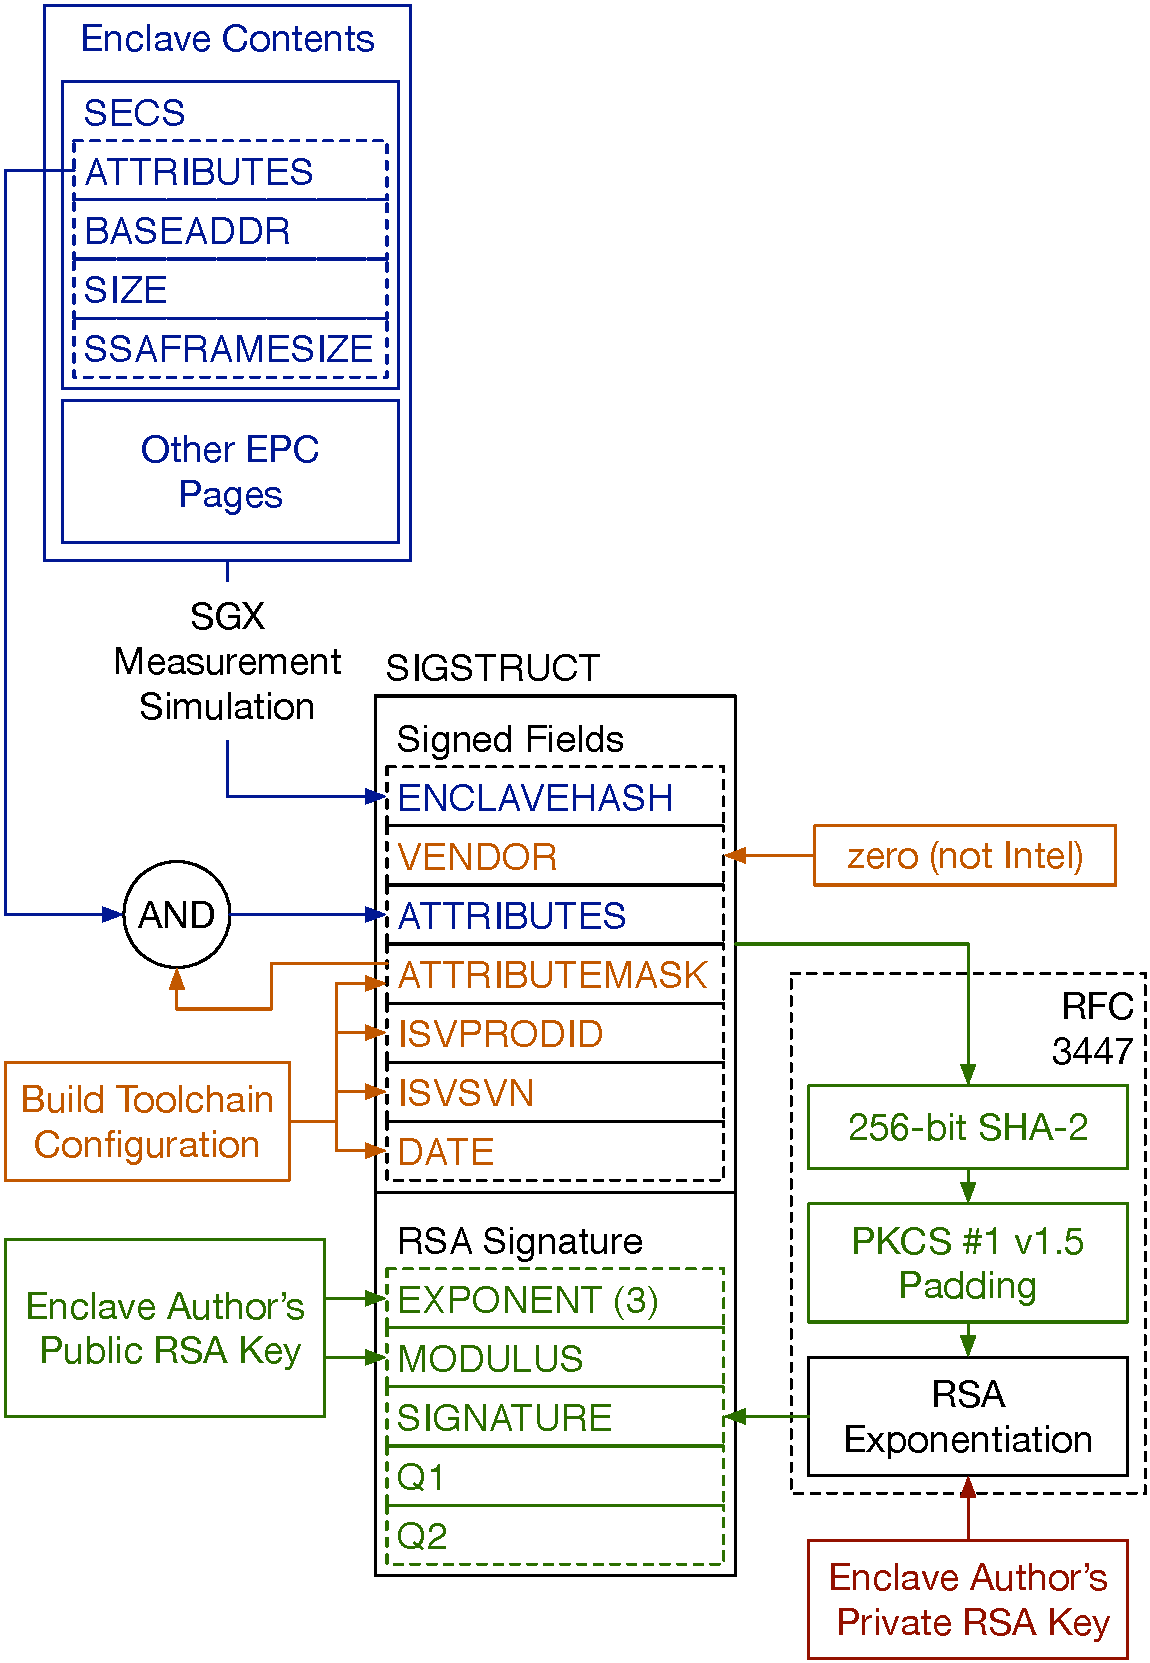
\includegraphics[width=85mm]{figures/sgx_sigstruct.pdf}
  \caption{
    An enclave's Signature Structure (SIGSTRUCT) is intended to be generated by
    an enclave building toolchain that has access to the enclave author's
    private RSA key.
  }
  \label{fig:sgx_sigstruct}
\end{figure}

SIGSTRUCT has a collection of fields, the most interesting of which are
presented in Table~\ref{fig:sgx_sigstruct_info}, and an RSA signature, which
uses the representation in Table~\ref{fig:sgx_sigstruct_rsa}.

\begin{table*}[hbt]
  \centering
  \begin{tabularx}{\textwidth}{| l | r | X |}
  \hline
  \textbf{Field} & \textbf{Bytes} & \textbf{Description} \\
  \hline
  VENDOR & 4 & Zero for non-Intel enclaves. Set to the special value
               \texttt{0x8086} for Intel enclaves.  \\
  \hline
  DATE & 4 & The enclave's build date, in hexadecimal format. Example:
             \texttt{0x20160129} \\
  \hline
  ATTRIBUTES & 16 & Constrains the ATTRIBUTE field of the enclave's SECS. \\
  \hline
  ATTRIBUTEMASK & 16 & Constrains the ATTRIBUTE field of the enclave's SECS. \\
  \hline
  ENCLAVEHASH & 32 & The enclave's measurement~(\S~\ref{sec:sgx_mrenclave}) \\
  \hline
  ISVPRODID & 32 & Product ID assigned by the enclave's author \\
  \hline
  ISVSVN & 32 & Security version number (SVN) assigned by the enclave's
                author \\
  \hline
  \end{tabularx}
  \caption{
    A subset of the fields in an enclave Signature Structure (SIGSTRUCT) whose
    authenticity is guaranteed by the RSA signature.
  }
  \label{fig:sgx_sigstruct_info}
\end{table*}

\begin{table*}[hbt]
  \centering
  \begin{tabularx}{\textwidth}{| l | r | X |}
  \hline
  \textbf{Field} & \textbf{Bytes} & \textbf{Description} \\
  \hline
  MODULUS & 384 & The modulus $m$ of the RSA signing key. \\
  \hline
  EXPONENT & 4 & The public exponent $e$ of the RSA signing key. SGX only
                 supports the exponent 3. \\
  \hline
  SIGNATURE & 384 & The RSA signature $s = M ^ e \bmod m$ over the SIGSTRUCT
                    fields \\
  \hline
  Q1 & 384 & $q_1$ value used to verify the RSA signature.
             (Explained in \S~\ref{sec:sgx_rsa_check}) \\
  \hline
  Q2 & 384 & $q_2$ value used to verify the RSA signature.
             (Explained \S~\ref{sec:sgx_rsa_check}) \\
  \hline
  \end{tabularx}
  \caption{
    The format of the RSA signature used in the enclave Signature Structure
    (SIGSTRUCT).
  }
  \label{fig:sgx_sigstruct_rsa}
\end{table*}

According to the SDM, the RSA signature in SIGSTRUCT is computed using the
method described in RFC 3447~\cite{jonsson2003pkcsv21}, using 256-bit
SHA-2~\cite{fips2015shs} as the hash function that reduces the input size, and
the padding method described in PKCS \#1 v1.5~\cite{kaliski1998pkcs1v15}. The
SGX implementation only supports 3072-bit RSA keys whose public exponent is 3.
The key size is likely chosen to meet FIPS'
recommendation~\cite{fips2012keysize}, whereas the exponent limitation opens up
the possibility to use the efficient signature verification algorithm described
in \S~\ref{sec:sgx_rsa_check}. The efficient algorithm also requires the fields
Q1 and Q2 in the RSA signature, which are also described in
\S~\ref{sec:sgx_rsa_check}.

The RSA signature in a SIGSTRUCT is verified by the SGX implementation when the
structure is used in an \texttt{EINIT}~(\S~\ref{sec:sgx_einit_overview})
invocation. The 256-bit SHA-2 hash of the EXPONENT field in the SIGSTRUCT is
also copied into the MRSIGNER field in the enclave's SECS. This value, referred
to as MRSIGNER throughout the SGX documentation, becomes the cryptographic
identity of the enclave's author. The ISVPRODID and ISVSVN fields from
SIGSTRUCT are also copied into the enclave's SECS. The role of these fields
will be revealed in \S~\ref{sec:sgx_egetkey}.


% Enclave Signature Structure (SIGSTRUCT): SDM S 38.13
% EINIT: SDM S 41.3

The SDM description of the VENDOR field in the section dedicated to SIGSTRUCT
suggests that the field is essentially used to distinguish between special
enclaves signed by Intel, which get a value of 0x8086, and everyone else's
enclaves, which get a VENDOR value of zero. However, the \textit{EINIT}
pseudocode seems to imply that the SGX implementation only checks that
VENDOR is either zero or 0x8086.


% Security Version Numbers: SDM S 39.4.2
% Enclave Security Version: SDM S 39.4.2.1

\subsubsection{Enclave Attributes}
\label{sec:sgx_attributes}

The ATTRIBUTES and ATTRIBUTESMASK fields in the SIGSTRUCT are used to restrict
the values of the ATTRIBUTES field in an enclave's SECS. \texttt{EINIT} refuses
to initialize an enclave using a SIGSTRUCT if the bitwise AND between the
ATTRIBUTES field in the enclave's SECS and the ATTRIBUTESMASK field in the
SIGSTRUCT does not equal the SIGSTRUCT's ATTRIBUTES field.

The restriction on ATTRIBUTES seems redundant for SGX enclaves that participate
in software attestation, because the SGX attestation signature includes the
value of the SECS' ATTRIBUTES field, so an enclave built with an undesirable
ATTRIBUTES value would be rejected during the attestation process.

% SECS.ATTRIBUTES.XFRM: SDM S 42.7.2.1

However, the ATTRIBUTES restriction does play a significant role for the
special enclaves signed by Intel, such as the Launch Enclave and the Quoting
Enclave. These enclaves gain access to SGX's secret keys without participating
in software attestation, and therefore must rely on another protection
mechanism. If \texttt{EINIT} would not enforce the ATTRIBUTES restrictions
expressed in SIGSTRUCT, malicious system software may be able to subvert a
special enclave's security checks by building the enclave with an unexpected
ATTRIBUTES value. For example, setting the XFRM
sub-field~(\S~\ref{sec:sgx_ssa}) to an unexpected value may enable
architectural extensions that the enclave wat not designed to handle.


\subsubsection{Enclave Key Generation}
\label{sec:sgx_egetkey}

% Keys: SDM S 39.4.3



% Security Version Numbers: SDM S 39.4.2
% Hardware Security Version: SDMS S 39.4.2.2

\subsubsection{License Verification}
\label{sec:sgx_launch_enclave}

% EINIT Token Structure (EINITTOKEN): SDM S 38.14

\begin{figure}[hbt]
  \centering
  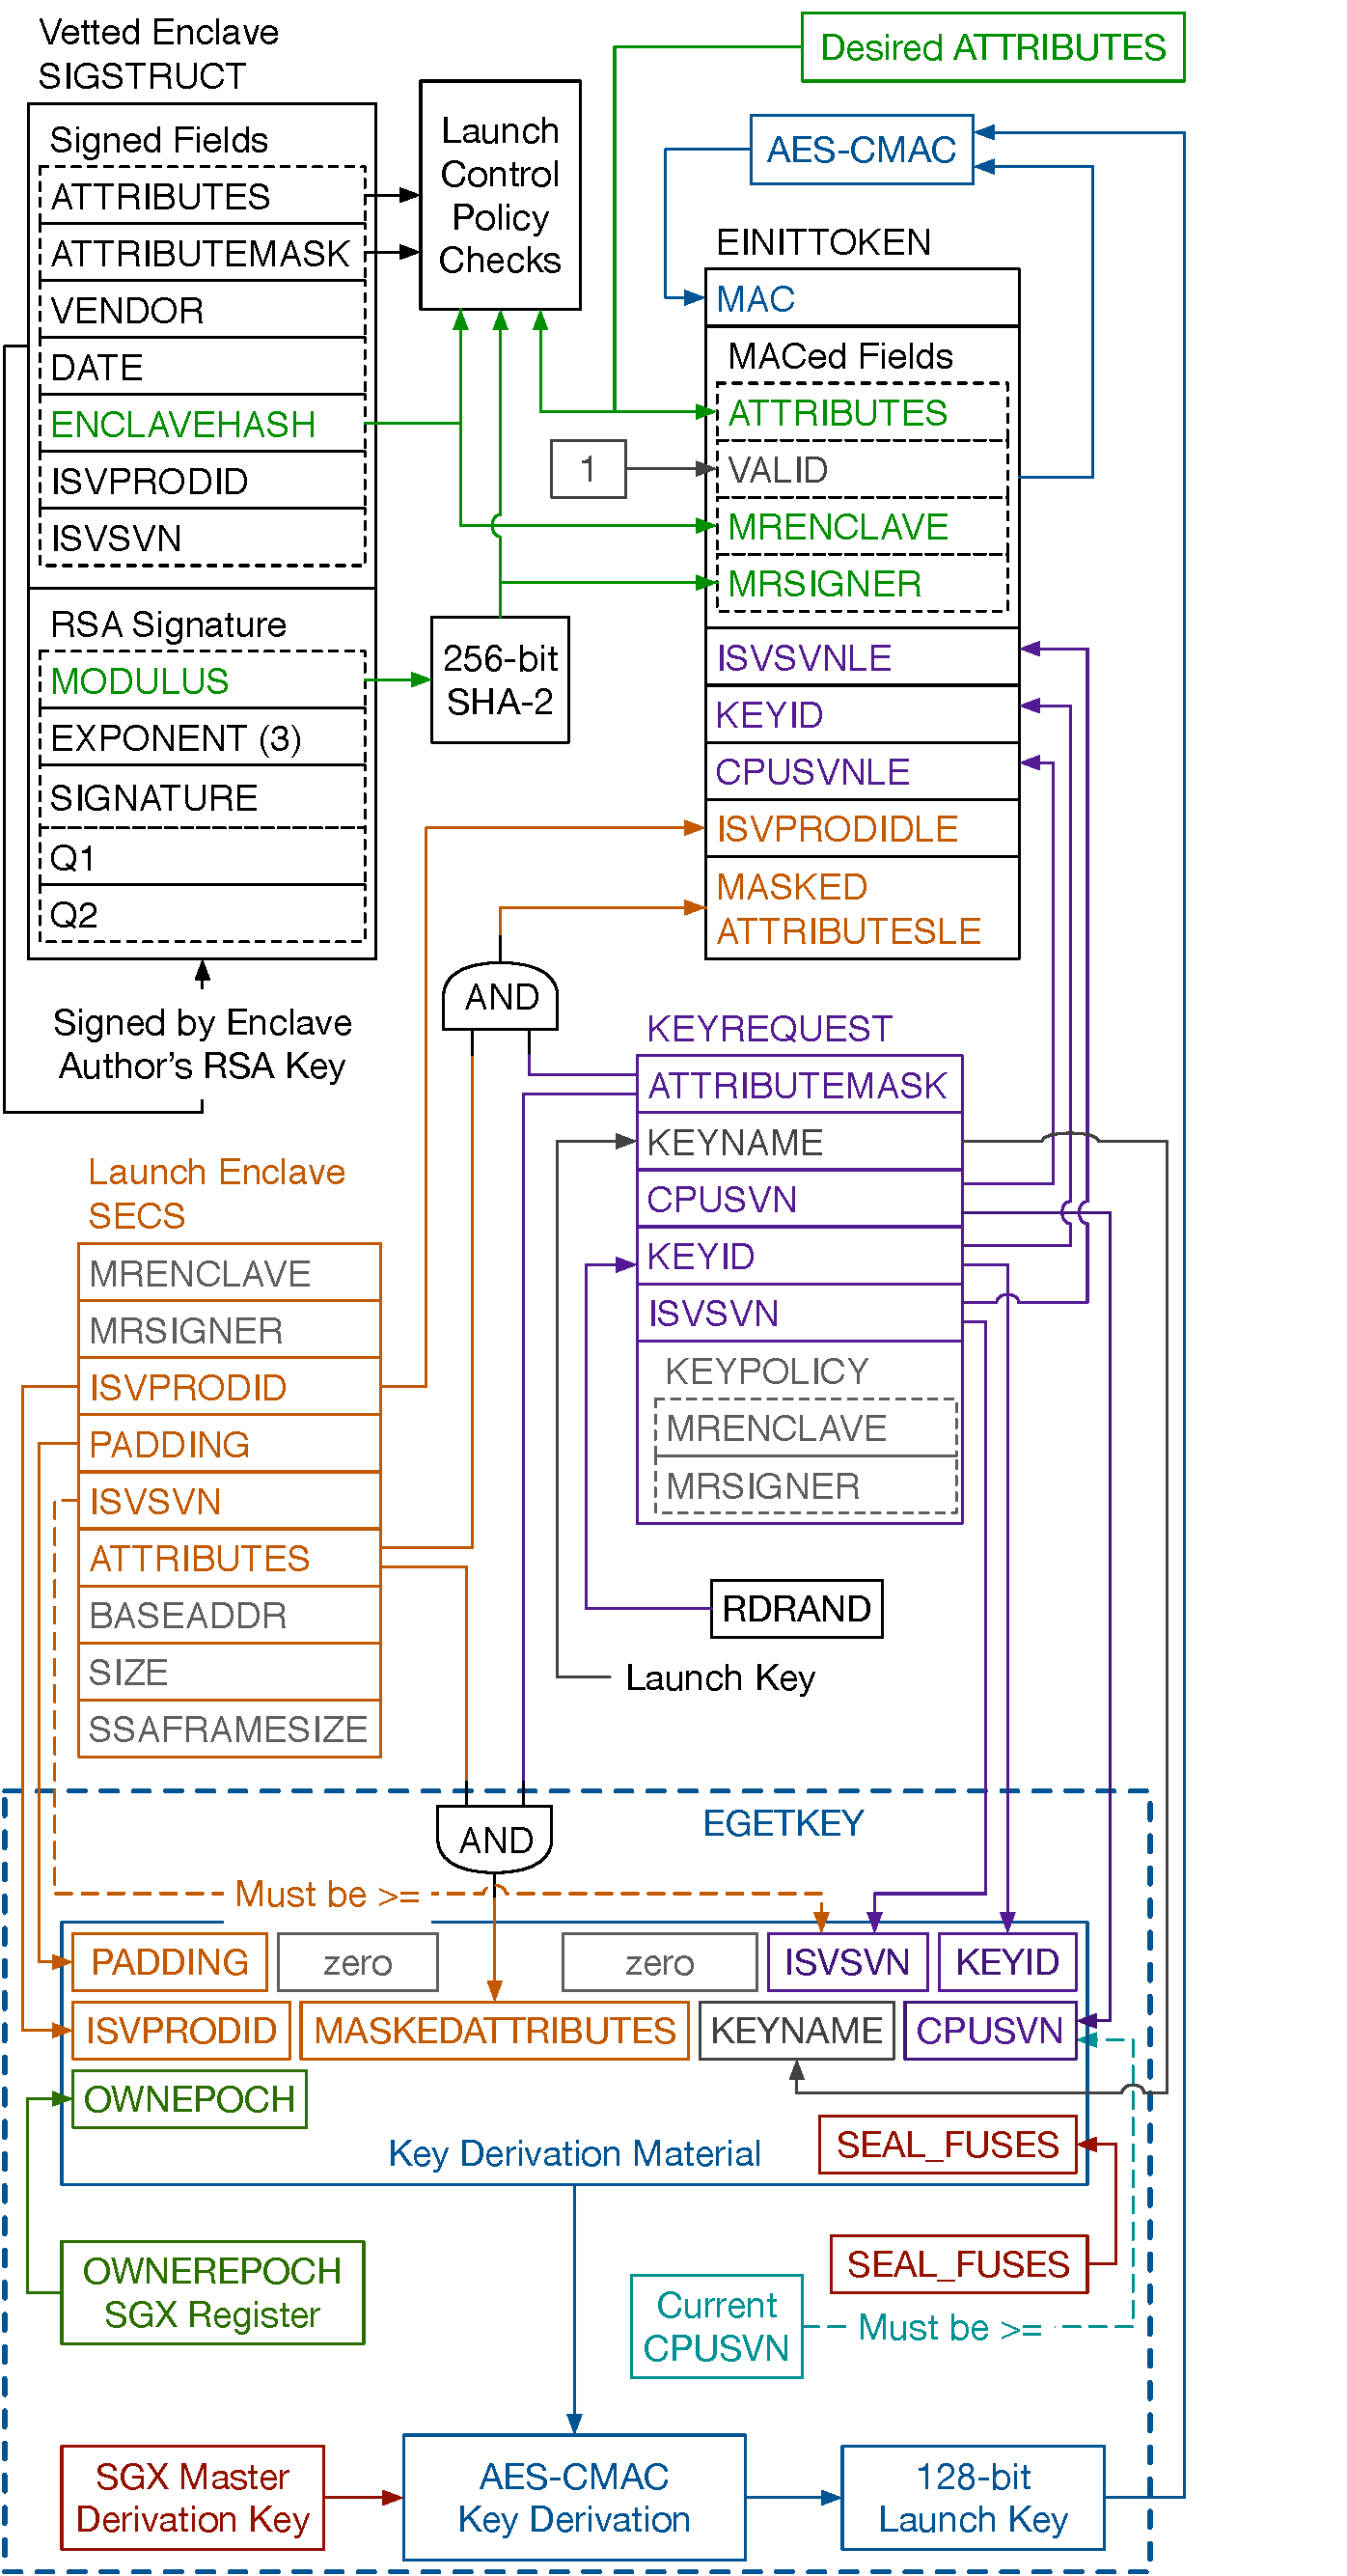
\includegraphics[width=87mm]{figures/sgx_einittoken.pdf}
  \caption{
    The SGX Launch Enclave computes the EINITTOKEN.
  }
  \label{fig:sgx_einittoken}
\end{figure}

The SDM states that the MAC that protects EINITTOKEN's authenticity is computed
using a block cipher-based MAC~(CMAC,~\cite{fips2005cmac}), but stops short of
specifying the underlying cipher. One of the SGX papers~\cite{anati2013sgx}
states that SGX implementation uses a CMAC based on 128-bit AES.



\subsubsection{Inter-Enclave Attestation}
\label{sec:sgx_ereport}

The enclave asks the CPU to produce an \textit{enclave report}, which contains
the attestation challenge, the enclave's measurement value, an
enclave-generated 256-byte message, and an HMAC
 with a symmetric key shared between the CPU and a special
\textit{signing enclave} produced by Intel. The untrusted system software
executes the signing enclave, which verifies the report and produces an
\textit{attestation signature} that covers the challenge and the enclave's
measurement.


\subsubsection{Enclave Initialization}
\label{sec:sgx_einit}

% MRSIGNER: SDM S 39.4.1.2

\texttt{EINIT}~(\S~\ref{sec:sgx_einit_overview}) requires the virtual address
of the SIGSTRUCT associated with the enclave to be initialized. The instruction
checks the validity of SIGSTRUCT's contents, and refuses to proceed if it
detects inconsistencies. For example, \texttt{EINIT} verifies the RSA
signature and returns an error code if the signature is invalid.

\texttt{EINIT} computes a 256-bit SHA-2 hash of the RSA exponent in the
enclave's SIGSTRUCT, and writes it into the MRSIGNER field in the enclave's
SECS. For this reason, the RSA exponent's hash is referred to as MRSIGNER
throughout the SGX documentation. This value is the cryptographic identity of
the enclave's author.

The \texttt{EINIT} instruction also copies the ISVPRODID and ISVSVN fields from
SIGSTRUCT into the enclave's SECS. In the scope of SGX's key generation
feature, which will be discussed in \S~\ref{sec:sgx_egetkey}, all the enclaves
that have the same MRSIGNER and ISVPRODID represent different versions of the
same software, and are ordered according to the value of the ISVSVN field.
Higher ISVSVN values identify newer enclave versions that potentially fix
security vulnerabilities found in the older versions.


\subsubsection{The Quoting Enclave}
\label{sec:sgx_quoting_enclave}

